\chapter{Data Collection and Understanding}

data collection and understanding play a pivotal role in extracting meaningful insights and deriving accurate conclusions.
The success of any analytical endeavor heavily relies on the quality, comprehensiveness, and relevance of the data used.
In the case of carbon emissions in maritime shipping, gathering and understanding the data is crucial for capturing the intricacies of this complex domain.
By exploring various data sources from industry databases, a comprehensive dataset can be acquired, encompassing diverse dimensions of carbon emissions in the maritime sector.
Furthermore, understanding the structure, variables, and limitations of the collected data is essential for ensuring the validity and reliability of subsequent analyses.
This includes examining the completeness of data, identifying any biases or data gaps, and verifying the accuracy of measurements.
Ultimately, a thorough and informed understanding of the data sets the foundation for conducting rigorous data analysis and generating actionable insights for addressing carbon emission challenges in maritime shipping.

Collaboration with Astrup Fearnleys Code has been instrumental in enhancing my research on carbon emissions in maritime shipping.
As a leading firm in the maritime shipping industry, their expertise and industry connections have provided me with invaluable support and access to crucial datasets.
Specifically, through their collaboration, I was able to gain access to two significant datasets: Automatic Identification System (AIS) data and IHS dataset.
Collaborating with Astrup Fearnleys Code and leveraging their industry expertise has not only provided me with valuable datasets but also allowed me to gain insights into the complex dynamics of the maritime shipping industry.

\newpage

\section{IHS Markit dataset}

The IHS Markit dataset provides valuable vessel specification data for big data analysis in maritime shipping.
This dataset offers comprehensive information on vessel characteristics, including dimensions, tonnage, engine capacity, and ownership.
By leveraging this dataset, researchers can gain insights into the diverse specifications of vessels operating in the maritime industry.

Analyzing vessel specifications from the IHS Markit dataset allows for a deeper understanding of the maritime shipping landscape.
Researchers can explore correlations between vessel characteristics and various factors such as fuel efficiency, cargo capacity, or operational performance.
These insights can aid in optimizing vessel selection, fleet management, and decision-making processes related to vessel operations.

By utilizing the vessel specification data from the IHS Markit dataset, this research contributes to enhancing operational efficiency and optimizing vessel-related decisions in the maritime shipping industry.
This dataset equipps this research to identify trends and patterns in the maritime shipping industry related to vessel characteristics.
This comprehensive dataset serves as a robust foundation for my research, enabling me to draw meaningful conclusions and make data-driven recommendations for the future of the industry.

\begin{figure}[h]
    \centering
    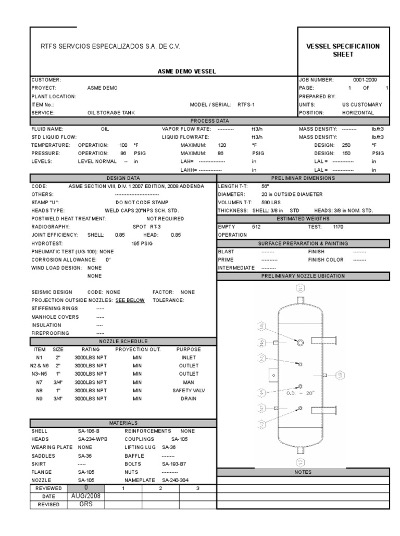
\includegraphics[width=0.5\textwidth]{images/vessel_specification.jpg}
    \caption{Vessel Specification Sheet \autocite{Itur}}
    \label{vessel_specification}
\end{figure}

\newpage


\section{The Automatic Identification System (AIS) dataset}

AIS (Automatic Identification System) was developed in the 1990s to enhance navigation safety and prevent ship collisions.
It allows ships equipped with AIS to communicate with each other and coastal authorities through VHF transmissions.
The International Maritime Organization (IMO) mandates that all international voyage ships above 300 gross tonnage and all passenger ships must have an AIS transmitter.
Governments and authorities in different nations also enforce AIS applications to improve safety and security.

\begin{figure}[h]
    \centering
    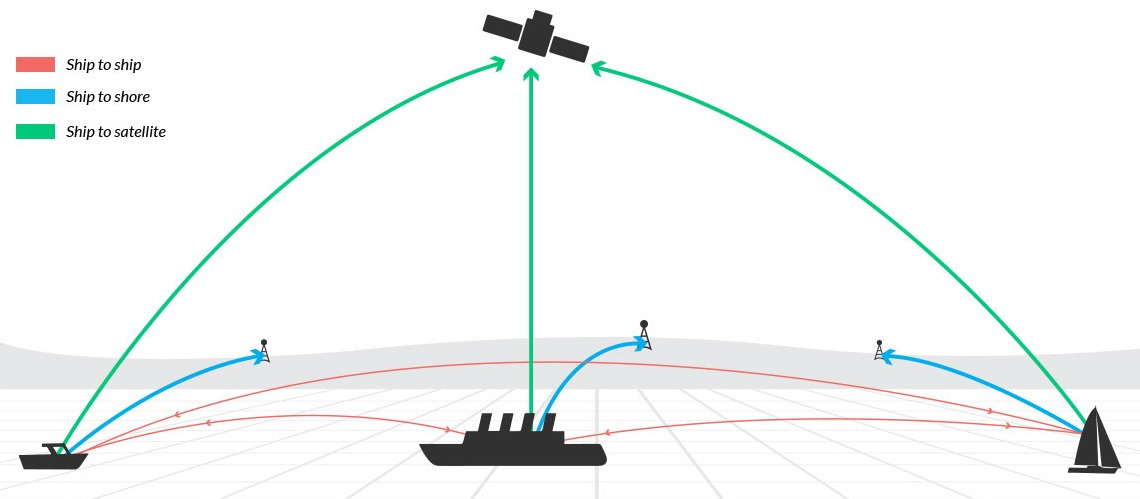
\includegraphics[width=0.7\textwidth]{images/ais.jpeg}
    \caption{Working of AIS}
    \label{ais}
\end{figure}

There are two types of AIS transceivers: Class A and Class B.
Class A transceivers broadcast more datafields and have higher reporting frequencies.
The information broadcasted by a Class A transceiver can be categorized into static information, dynamic information, and voyage-related information.
Dynamic information is automatically transmitted every 2-10 seconds when the ship is underway and every 3 minutes when anchored.
Static and voyage-related information are broadcasted every 6 minutes regardless of navigational status.
Class B transponders transmit a reduced set of data and have sparser reporting intervals compared to Class A transponders.


\begin{table}[ht]
    \centering
    \begin{tabular}{|l|l|p{0.5\linewidth}|}
        \hline
        \textbf{Data field}       & \textbf{Type} & \textbf{Description}                                                                      \\
        \hline
        AIS identity and location & Static        & Maritime Mobile Service Identity (MMSI) and the location of the system's antenna on board \\
        \hline
        Ship identity             & Static        & Ship name, IMO number, type, and call sign of the ship                                    \\
        \hline
        Ship size                 & Static        & Length and width of the ship                                                              \\
        \hline
        Ship position             & Dynamic       & Latitude and longitude (up to 0.0001 min accuracy)                                        \\
        \hline
        Speed                     & Dynamic       & Ranging from 0 knot to 102 knots (0.1 knot resolution)                                    \\
        \hline
        Rate of turn              & Dynamic       & Right or left (ranging from 0 to 720° per minute)                                         \\
        \hline
        Timestamp                 & Dynamic       & Timestamp of the message in UTC                                                           \\
        \hline
    \end{tabular}
    \caption{AIS message data fields \autocite{perez2009automatic}}
    \label{tab:ais_message}
\end{table}


Table \ref{tab:ais_message} shows the data fields transmitted by AIS messages.
Combining AIS data with other databases can provide additional information.
For example, port-to-port average speed can be calculated based on voyage distance and time stamps reported at the two ports.
Cargo weight can be estimated using draught and ship sizes. Technical ship specifications, such as DWT (deadweight tonnage), capacity, design speed, and design draught, can be obtained from fleet databases using the IMO number.
Port-to-port bunker consumption can be estimated based on speed, distance, and technical ship specifications like DWT and capacity \autocite{yang2019big}.


(Write more about the dataset source and how it is collected)


